\section{Трансформация пространства}
Рассмотрим подробнее каждое из пространств и подумаем как именно можно их сужать и какие гиперпараметры могут быть. Здесь мы рассотрим это с логической точки зрения, качетсвенно на практике мы рассмотрим в следующем параграфе
\subsection{Входное пространство}
Рассмотрим более подробно сужение на входном простратсве, насколько мы знаем $X$ представляет собой тензор размера (28, 28). При использовании дискретизации на 2 значения (0, 1) полученное простраство имеет размер $2^{28 * 28}$, что очень много, поэтому перед дискретизацией мы будем использовать пуллинги. Рассмотрим примеры входных пространств:
\begin{center}
    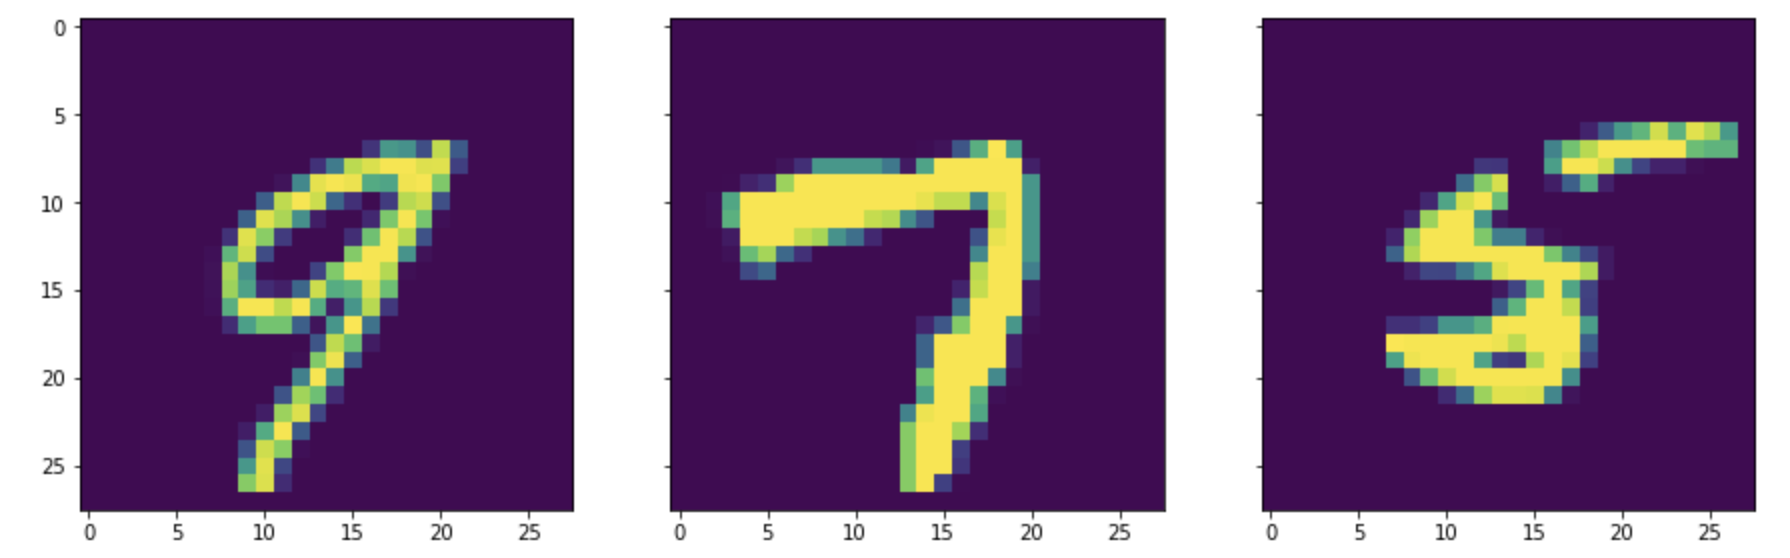
\includegraphics[scale=0.5]{images/plt_input.png}
\end{center}
Как видно картинки представляют собой узкие линии значений близких к 1. Соответственно градиент по картинке высокий. Соответственно при использовании усреднения картинка получится размытая и не будет обладать большим количеством информации о том, что было изначально нарисовано на картинке. \\
Пример использования $Average Pooling$ с окном (7, 7) c навешенной дискретизацией  $discrete$:
\begin{gather}
\begin{aligned}  
discrete(x) = 
\begin{cases}
    0, & \text{if } x\leqslant 0.5\\
    1,              & \text{otherwise}
\end{cases}
\end{aligned}
\end{gather}
\begin{center}
    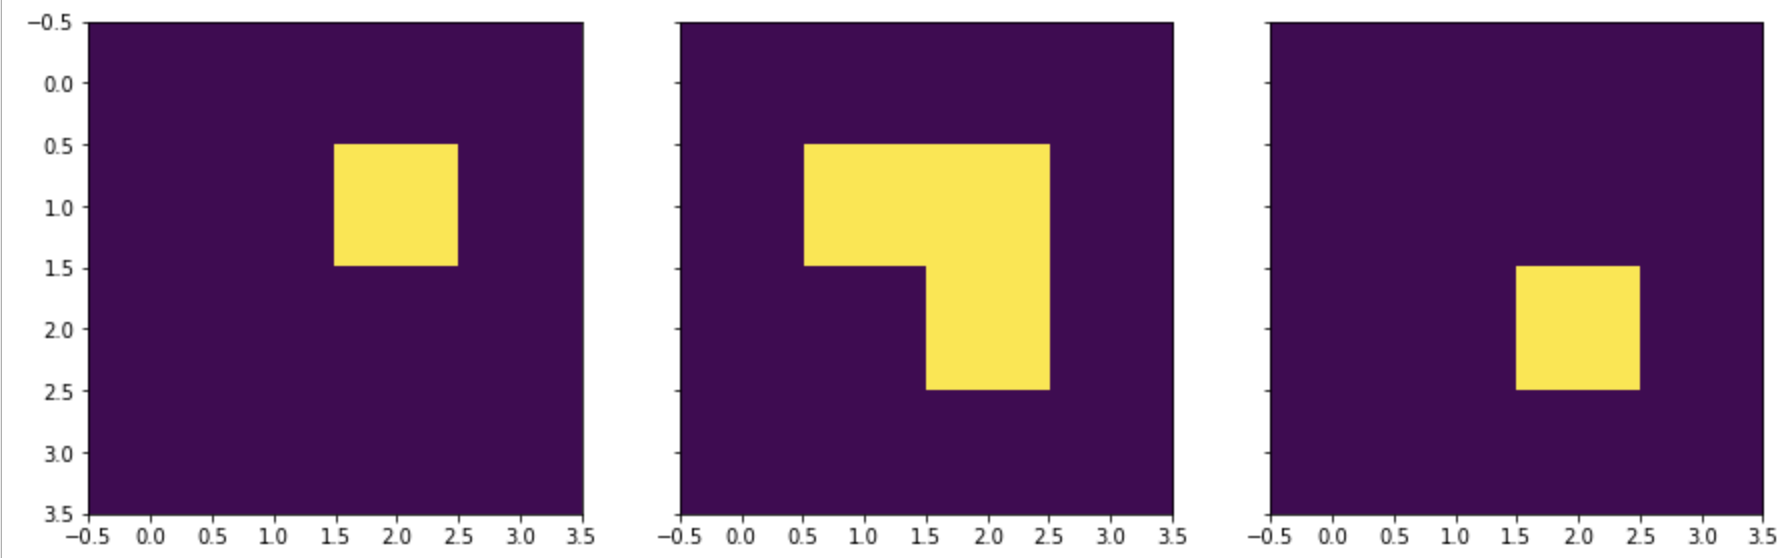
\includegraphics[scale=0.5]{images/plt_arg_7.png}
\end{center}
Праклика показывает что полученное представление не переносит много информации с входного пространства. Если выбирать в окне максимум полученное изображение не будет размываться, а значит будет сохранятся больше информации. \\
Пример использования $Max Pooling$ с окном (7, 7) c навешенной дискретизацией  $discrete$:
\begin{center}
    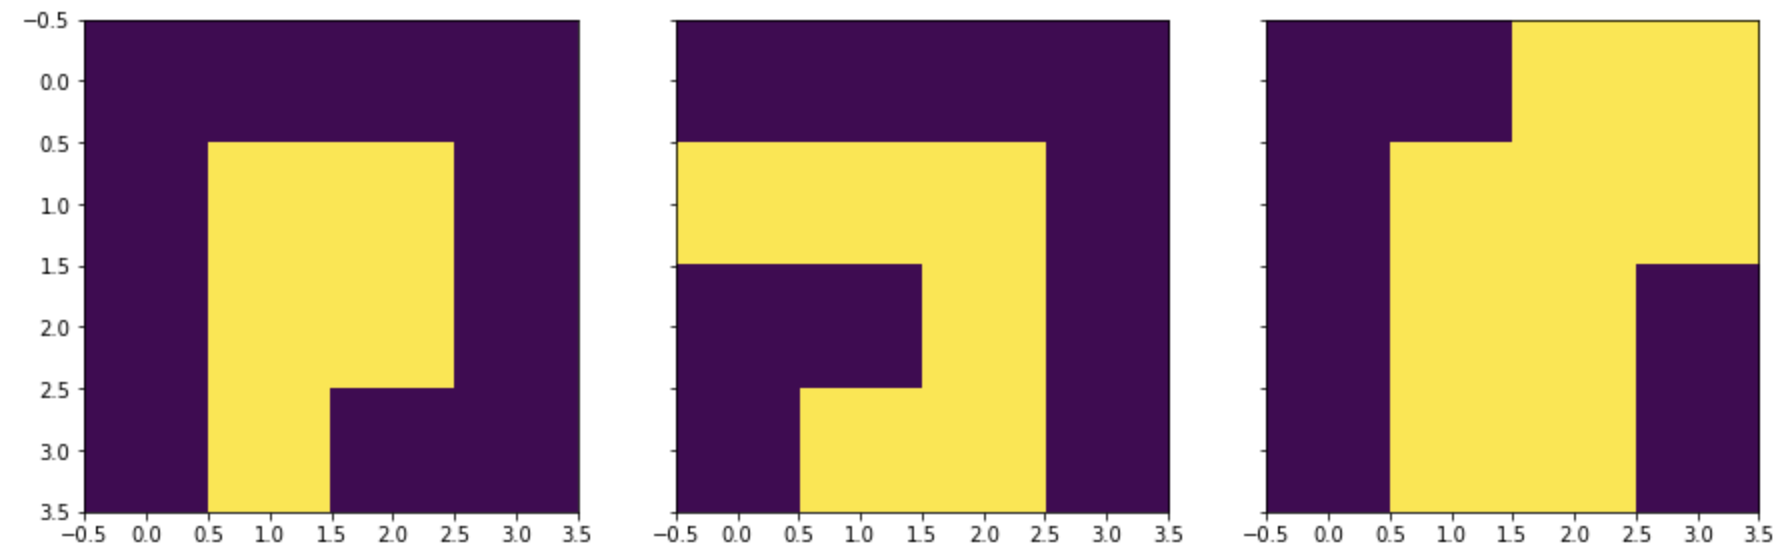
\includegraphics[scale=0.5]{images/plt_max_7.png}
\end{center}
В качетстве увеличения информации имеет смысл уменьшить окно пуллинга. При этом пространство будет больше и больше вероятность инъективности отображения, но количество перетекаемой информации также увеличится. \\
Пример использования $Max Pooling$ с окном (4, 4) c навешенной дискретизацией  $discrete$:
\begin{center}
    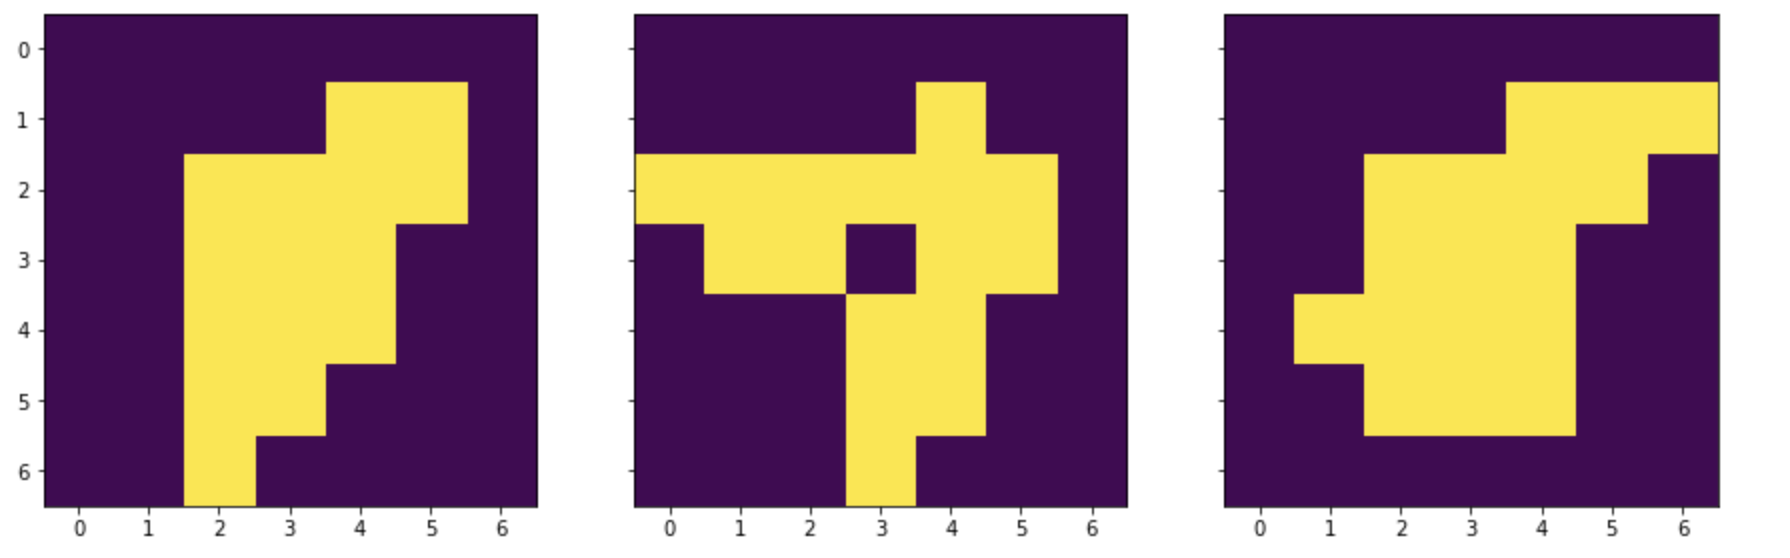
\includegraphics[scale=0.5]{images/plt_max_4.png}
\end{center}

\subsection{Латентное финальное простраство}
Здесь мы рассотрим пространство $Z_3$ которое является выходным слоем сети. Во время обучения от данного слоя берется функция $Softmax$ и уже сравнивается с $one hot$ векторов метки изобажения. Соответственно в пространстве $Z_3$ нам не важны сами значения, нам важен их порядок и индекс наибольшего значения, так как после применения операции $Softmax$ наибольшее значение из всех станет близки к 1, а все остальные близки к 0
\begin{gather}
\begin{aligned}  
softmax(x_i) \approx 
\begin{cases}
    1, & \text{if } i = max\_index\\
    0, & \text{if } i \neq max\_index
\end{cases}
\end{aligned}
\end{gather}
Поэтому нам не так важно распеделение на финальном слое, как важен порядок. Поэтому преобразование на финальном латентном пространстве будет функция $Softmax$.
\subsection{Промежуточные латентные пространства}
В качетсве примера возьмем устройство пространства $Z_1$, пространство $Z_2$ устроено аналогично, так как оно получается таким же образом, а имеено с помощью сверточного слоя. Напомним что пространство $Z_1$ имеет размерность $(dataset\_size, 16, 14, 14)$ \\
В качестве примера рассмотрим выход $z_1 \in Z_1$ - а именно результат свертки одной из входных картинок. Разложим тензор по всем 16 каналов: 
\begin{center}
    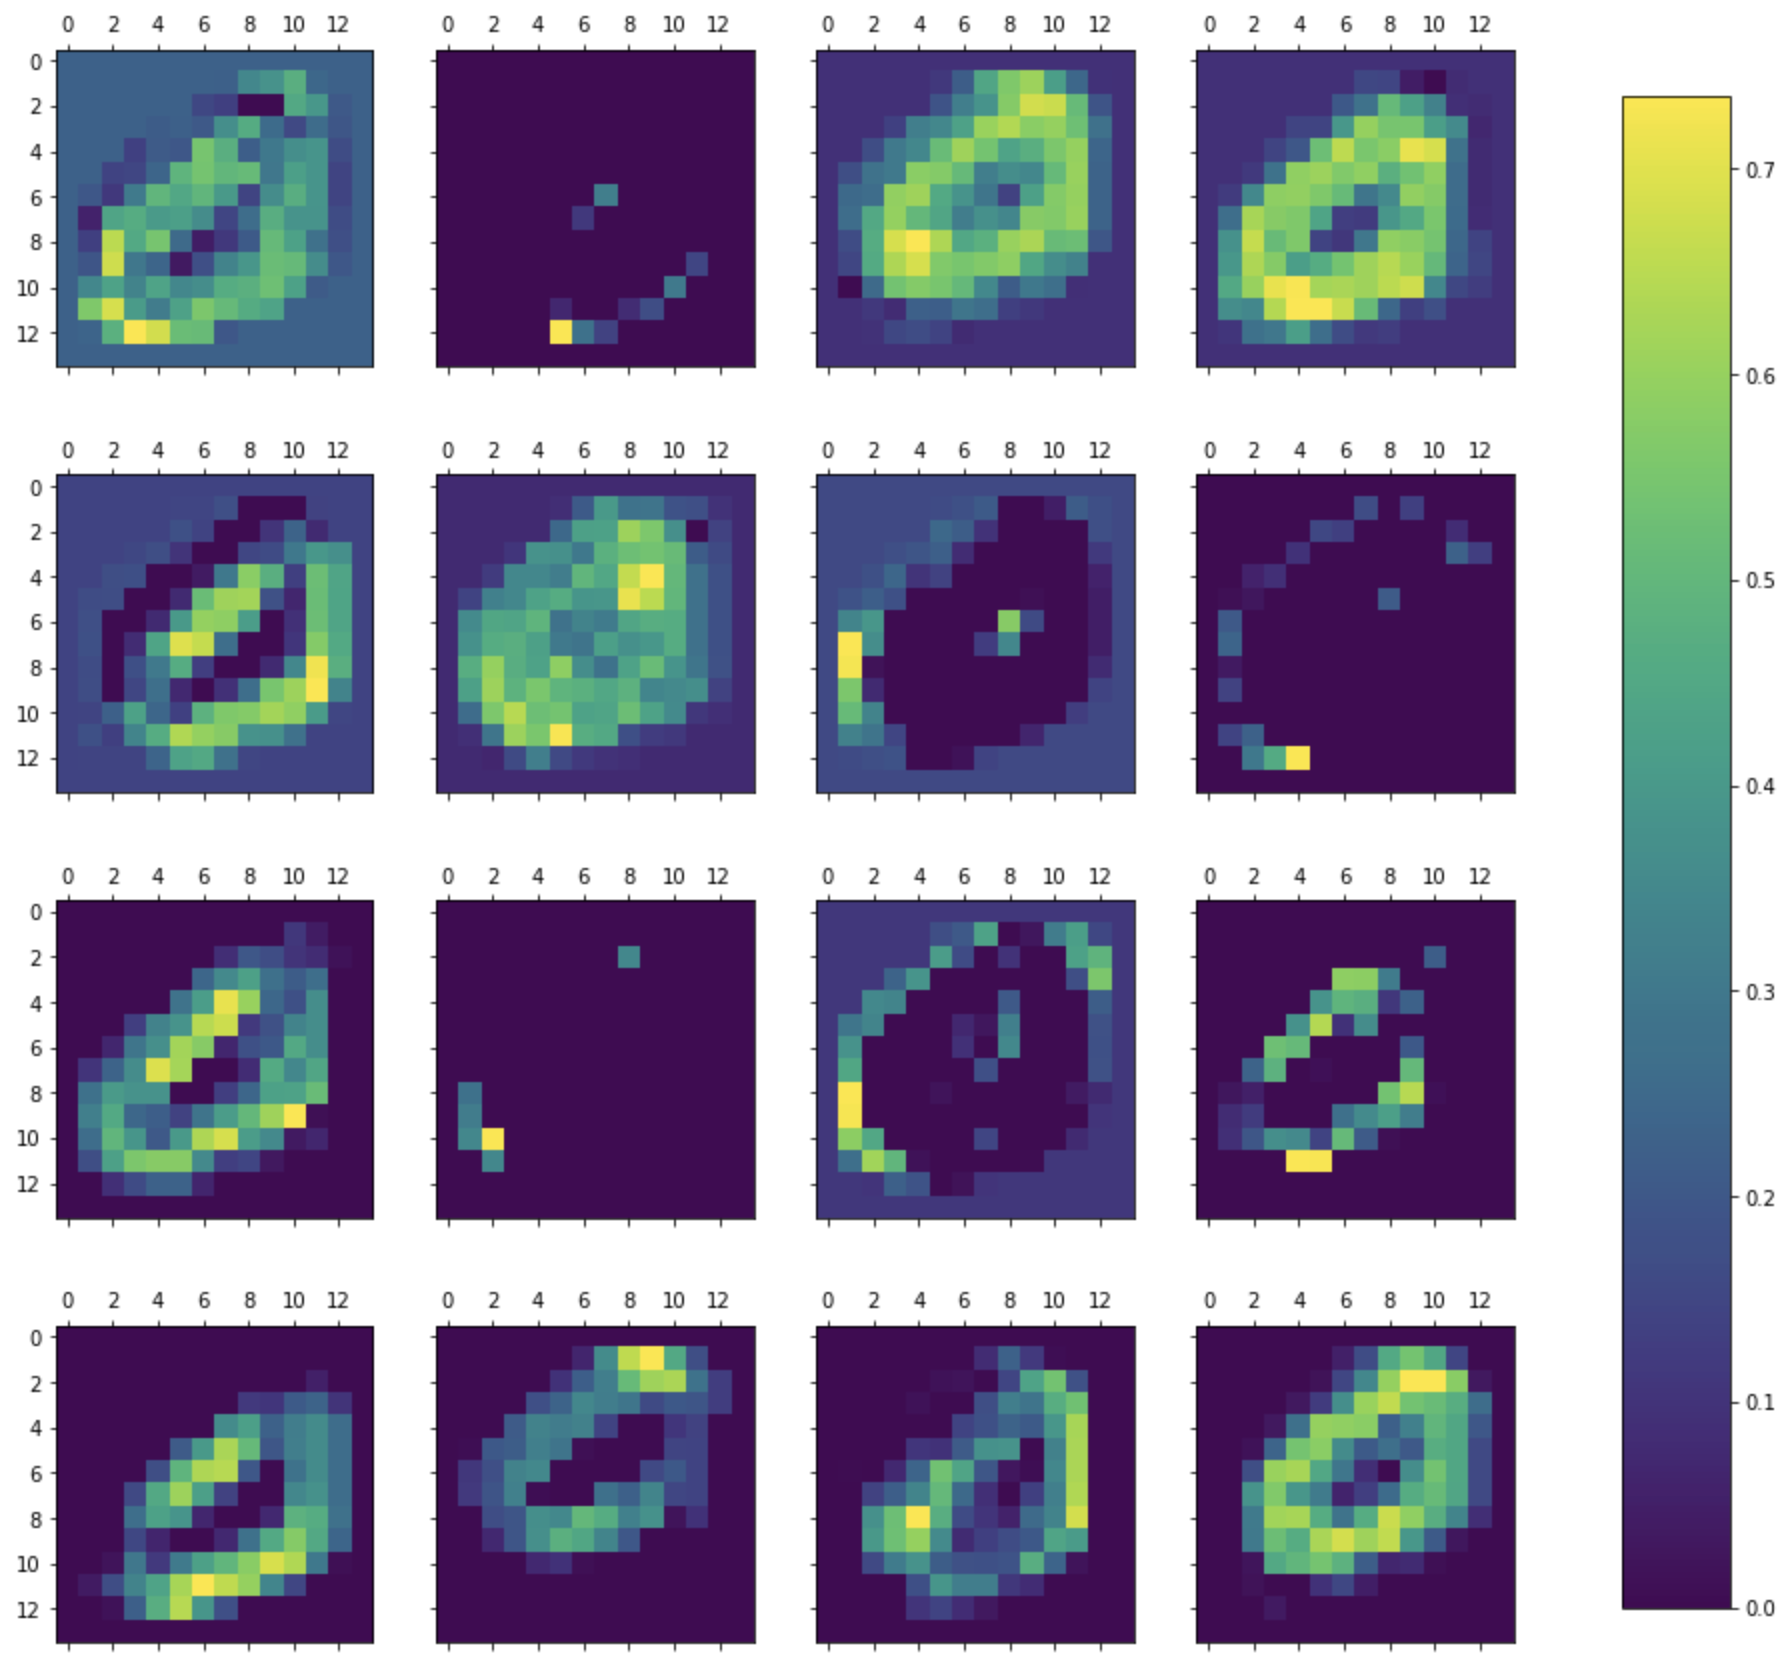
\includegraphics[scale=0.5]{images/plt_z1.png}
\end{center}
Как видно, каждый из 16ти различных каналов представляет собой такое же изображение, где каждая ячейка показывает как реагирует соответствующее окно на определенный фильтр, который сответствует данному каналу. С точки зрения информации нам важно какие места реагируют на различные свертки-фильтры, то есть нам важно понимать как утроены большие значения по признакам (зеленые, желтые на картинке). \\
Для дальнейшей дискретизации нам важно как распределены значения в пространстве по каждому призраку. Для этого посчитаем 0.01 квантиль ($min\_hidden\_border$) и 0.99 квантиль ($max\_hidden\_border$) для каждого из признаков по выборке:
\begin{center}
    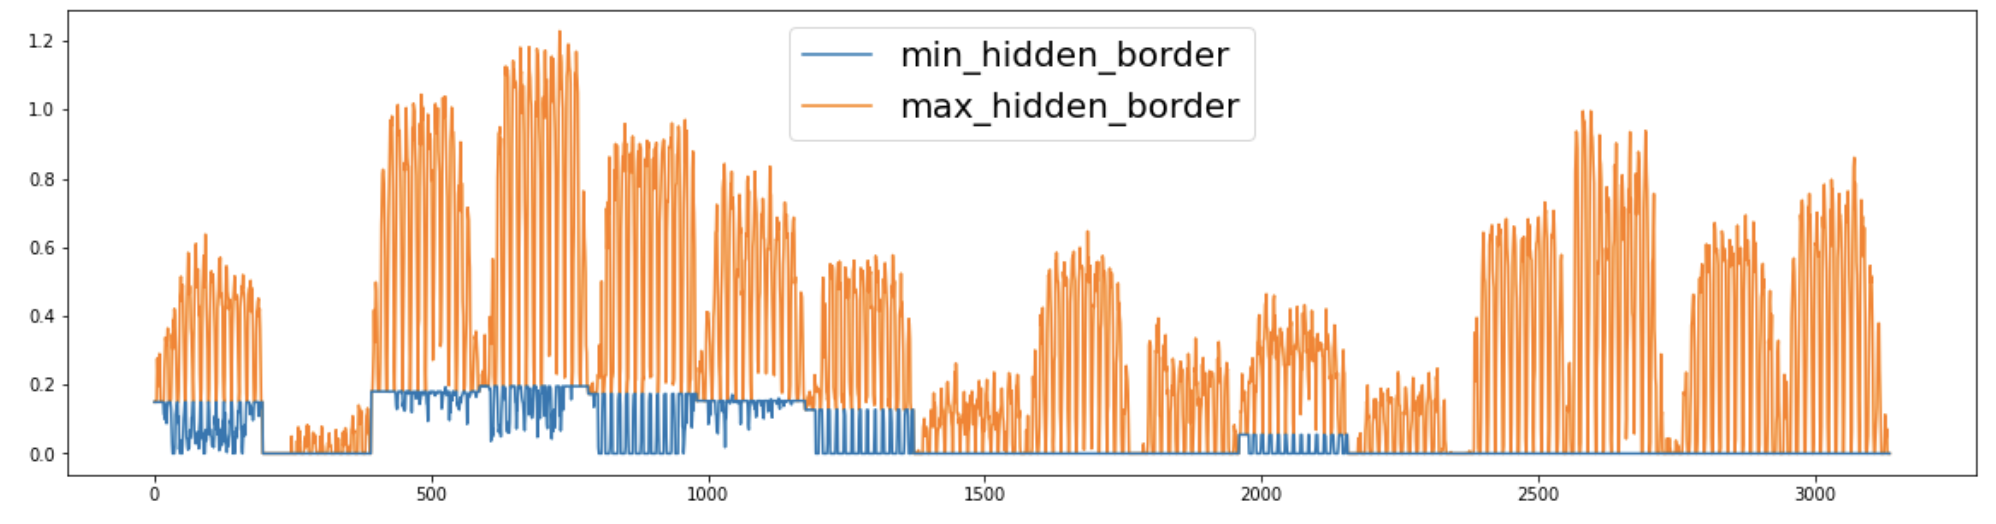
\includegraphics[scale=0.5]{images/z1_borders.png}
\end{center}
Также посчитаем среднее $hidden\_mean$ и дисперсию $hidden\_std$ по каждому признаку:
\begin{center}
    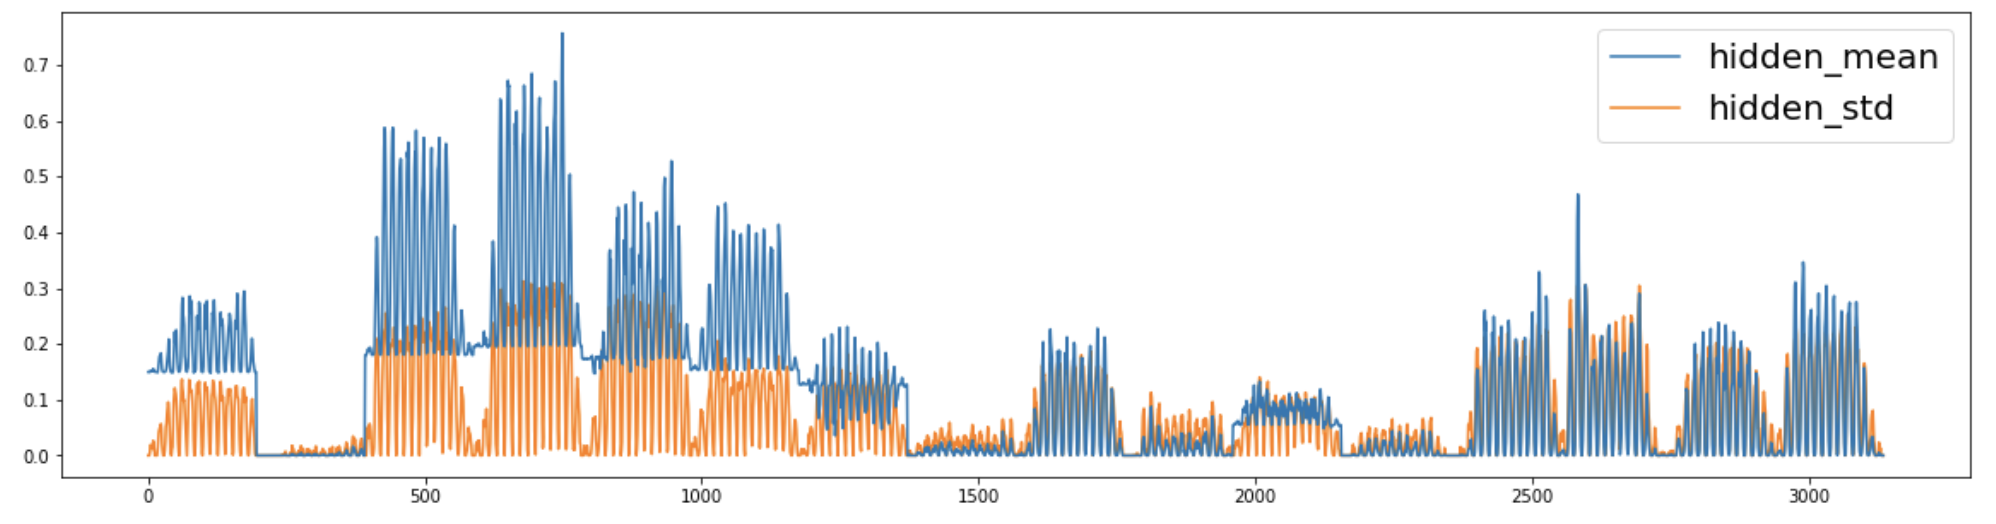
\includegraphics[scale=0.5]{images/z1_means.png}
\end{center}
Как видно распределение по каждому призаку отличаются, отсюда можно сделать вывод что при дискретизации значения к которым будут приближаться пространства будут для каждого признака различны и расчитываться из соответствующих для них $min\_hidden\_border$ и $max\_hidden\_border$. \\
Поскольку нам важно понимать как утроены места с большими значениями в качестве пуллинга будет использоваться $maxpool$, поскольку $avgpool$ будет делать значения более размытыми. Пример дискретизации с последовательным применением пуллинга и дискретизации, то есть дискретизация проводится по уже сжатой выборке:
\begin{center}
    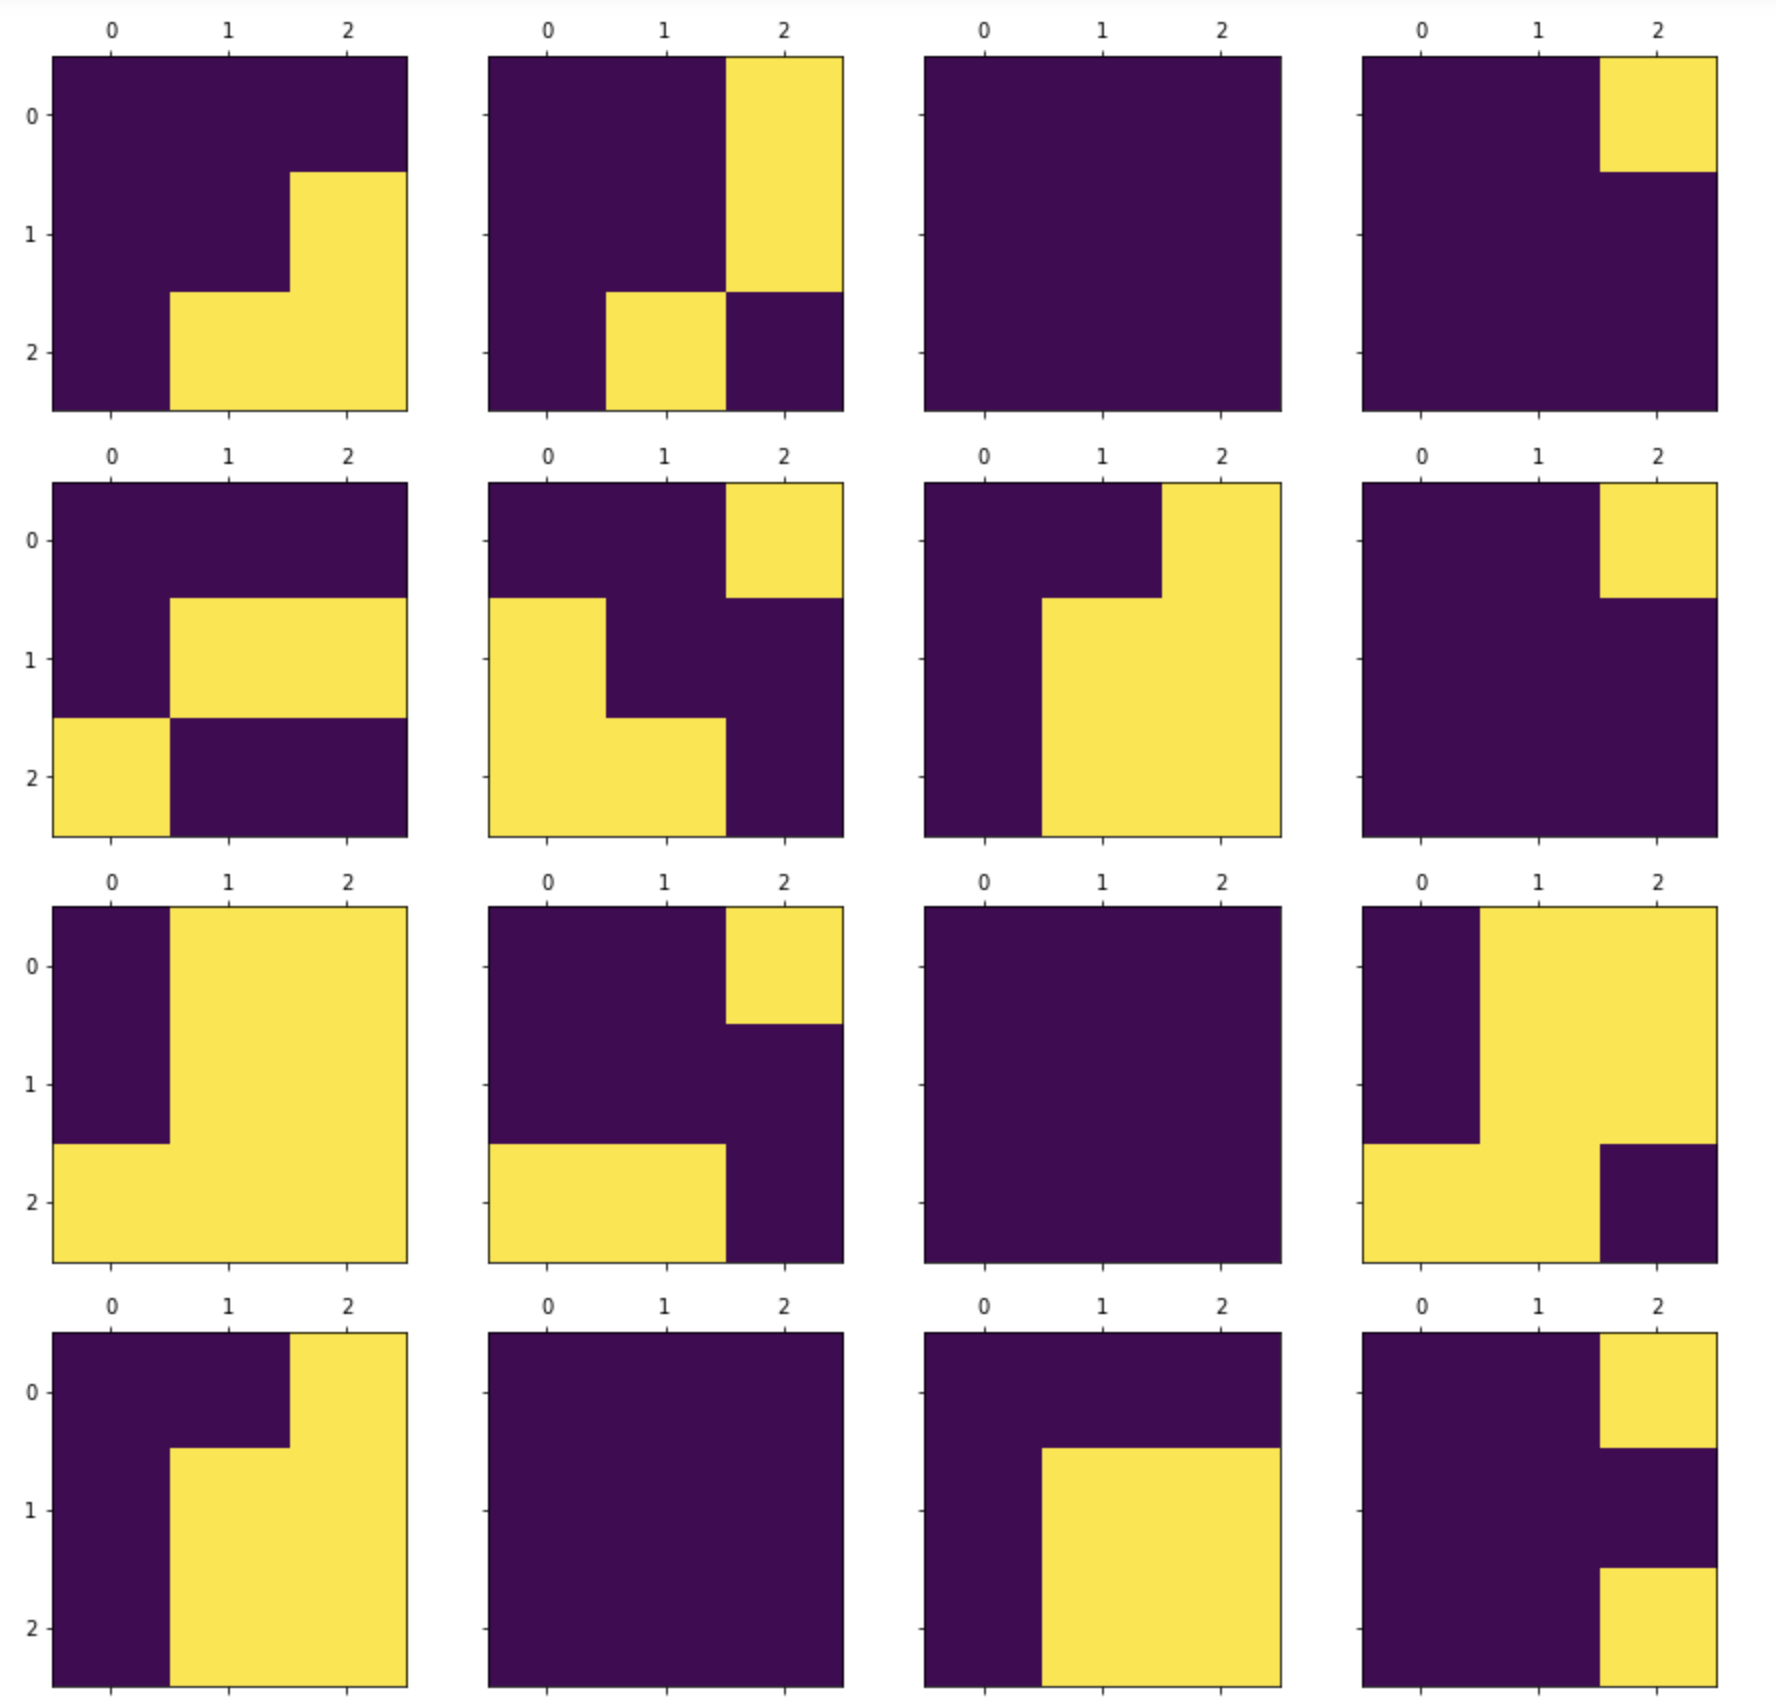
\includegraphics[scale=0.5]{images/z1_max_7.png}
\end{center}\
Аналогичную операцию сужения пространства будем проводить с следующем латентным пространством $Z_2$. Параметры пуллинга остаются гиперпараметрами и устанавливаются на валидации. При этом условие проводить $MaxPool2d$ или $MaxPool3d$ также остается гиперпараметром, так как каналы более независимы друг от друга чем значения внутри каждого канала. Но при этом при смешиваниии каналов дискретизация приводит к меньшему простанству и уменьшается риск инъективности отобрания. 




